\begin{tikzpicture}
\tikzset{frontier/.style={distance from root=150pt}}
    \Tree   [.{\textbf{Palabra}} 
[.{\textbf{\upshape S$_1$}} 
[[.\textit{Ataque} [.C$_1$ {\textit{t}} ] 
[.C$_2$ {\textit{r}} ]]] 
[.\textit{Rima}
[.\textit{Núcleo} [.C$_1$ {\textit{a}} ] ]
[.\textit{Coda}  [.C$_2$ {\textit{n}} ] 
[.C$_2$ {\textit{s}} ] ] ] ]
%
%
[.{\textbf{\upshape S$_2$}} 
[[.\textit{Ataque} [.C$_1$ {\textit{p}} ]] ]
[.\textit{Rima}
[.\textit{Núcleo}  [.S$_1$ {\textit{u}} ]
[.V {\textit{e}} ] ]
[.\textit{Coda} [.C$_1$ {\textit{s}} ] ]]]
%
%
[.{\textbf{\upshape S$_3$}} 
[[.\textit{Ataque} [.C$_1$ {\textit{t}} ] ]]
[.\textit{Rima}
[.\textit{Núcleo}  [.V {\textit{o}} ] ]]]
]
\end{tikzpicture}
